% Options for packages loaded elsewhere
\PassOptionsToPackage{unicode}{hyperref}
\PassOptionsToPackage{hyphens}{url}
%
\documentclass[
]{article}
\usepackage{amsmath,amssymb}
\usepackage{lmodern}
\usepackage{iftex}
\ifPDFTeX
  \usepackage[T1]{fontenc}
  \usepackage[utf8]{inputenc}
  \usepackage{textcomp} % provide euro and other symbols
\else % if luatex or xetex
  \usepackage{unicode-math}
  \defaultfontfeatures{Scale=MatchLowercase}
  \defaultfontfeatures[\rmfamily]{Ligatures=TeX,Scale=1}
\fi
% Use upquote if available, for straight quotes in verbatim environments
\IfFileExists{upquote.sty}{\usepackage{upquote}}{}
\IfFileExists{microtype.sty}{% use microtype if available
  \usepackage[]{microtype}
  \UseMicrotypeSet[protrusion]{basicmath} % disable protrusion for tt fonts
}{}
\makeatletter
\@ifundefined{KOMAClassName}{% if non-KOMA class
  \IfFileExists{parskip.sty}{%
    \usepackage{parskip}
  }{% else
    \setlength{\parindent}{0pt}
    \setlength{\parskip}{6pt plus 2pt minus 1pt}}
}{% if KOMA class
  \KOMAoptions{parskip=half}}
\makeatother
\usepackage{xcolor}
\usepackage[margin=1in]{geometry}
\usepackage{longtable,booktabs,array}
\usepackage{calc} % for calculating minipage widths
% Correct order of tables after \paragraph or \subparagraph
\usepackage{etoolbox}
\makeatletter
\patchcmd\longtable{\par}{\if@noskipsec\mbox{}\fi\par}{}{}
\makeatother
% Allow footnotes in longtable head/foot
\IfFileExists{footnotehyper.sty}{\usepackage{footnotehyper}}{\usepackage{footnote}}
\makesavenoteenv{longtable}
\usepackage{graphicx}
\makeatletter
\def\maxwidth{\ifdim\Gin@nat@width>\linewidth\linewidth\else\Gin@nat@width\fi}
\def\maxheight{\ifdim\Gin@nat@height>\textheight\textheight\else\Gin@nat@height\fi}
\makeatother
% Scale images if necessary, so that they will not overflow the page
% margins by default, and it is still possible to overwrite the defaults
% using explicit options in \includegraphics[width, height, ...]{}
\setkeys{Gin}{width=\maxwidth,height=\maxheight,keepaspectratio}
% Set default figure placement to htbp
\makeatletter
\def\fps@figure{htbp}
\makeatother
\setlength{\emergencystretch}{3em} % prevent overfull lines
\providecommand{\tightlist}{%
  \setlength{\itemsep}{0pt}\setlength{\parskip}{0pt}}
\setcounter{secnumdepth}{5}
\newlength{\cslhangindent}
\setlength{\cslhangindent}{1.5em}
\newlength{\csllabelwidth}
\setlength{\csllabelwidth}{3em}
\newlength{\cslentryspacingunit} % times entry-spacing
\setlength{\cslentryspacingunit}{\parskip}
\newenvironment{CSLReferences}[2] % #1 hanging-ident, #2 entry spacing
 {% don't indent paragraphs
  \setlength{\parindent}{0pt}
  % turn on hanging indent if param 1 is 1
  \ifodd #1
  \let\oldpar\par
  \def\par{\hangindent=\cslhangindent\oldpar}
  \fi
  % set entry spacing
  \setlength{\parskip}{#2\cslentryspacingunit}
 }%
 {}
\usepackage{calc}
\newcommand{\CSLBlock}[1]{#1\hfill\break}
\newcommand{\CSLLeftMargin}[1]{\parbox[t]{\csllabelwidth}{#1}}
\newcommand{\CSLRightInline}[1]{\parbox[t]{\linewidth - \csllabelwidth}{#1}\break}
\newcommand{\CSLIndent}[1]{\hspace{\cslhangindent}#1}
\ifLuaTeX
  \usepackage{selnolig}  % disable illegal ligatures
\fi
\IfFileExists{bookmark.sty}{\usepackage{bookmark}}{\usepackage{hyperref}}
\IfFileExists{xurl.sty}{\usepackage{xurl}}{} % add URL line breaks if available
\urlstyle{same} % disable monospaced font for URLs
\hypersetup{
  pdftitle={Different rules for binocular combination of luminance in cortical and subcortical pathways},
  pdfauthor={Federico G. Segala, Aurelio Bruno, Alex R. Wade \& Daniel H. Baker (+Myat? +Joel?)},
  hidelinks,
  pdfcreator={LaTeX via pandoc}}

\title{Different rules for binocular combination of luminance in cortical and subcortical pathways}
\author{Federico G. Segala, Aurelio Bruno, Alex R. Wade \& Daniel H. Baker (+Myat? +Joel?)}
\date{2022-09-22}

\begin{document}
\maketitle

\hypertarget{abstract}{%
\section{Abstract}\label{abstract}}

\hypertarget{introduction}{%
\section{Introduction}\label{introduction}}

\hypertarget{methods}{%
\section{Methods}\label{methods}}

\hypertarget{participants}{%
\subsection{Participants}\label{participants}}

\hypertarget{apparatus-stimuli}{%
\subsection{Apparatus \& Stimuli}\label{apparatus-stimuli}}

\hypertarget{procedure}{%
\subsection{Procedure}\label{procedure}}

\hypertarget{data-analysis}{%
\subsection{Data analysis}\label{data-analysis}}

Baker (2021)

\hypertarget{results}{%
\section{Results}\label{results}}

\hypertarget{experiment-1}{%
\subsection{Experiment 1}\label{experiment-1}}

\begin{figure}

{\centering 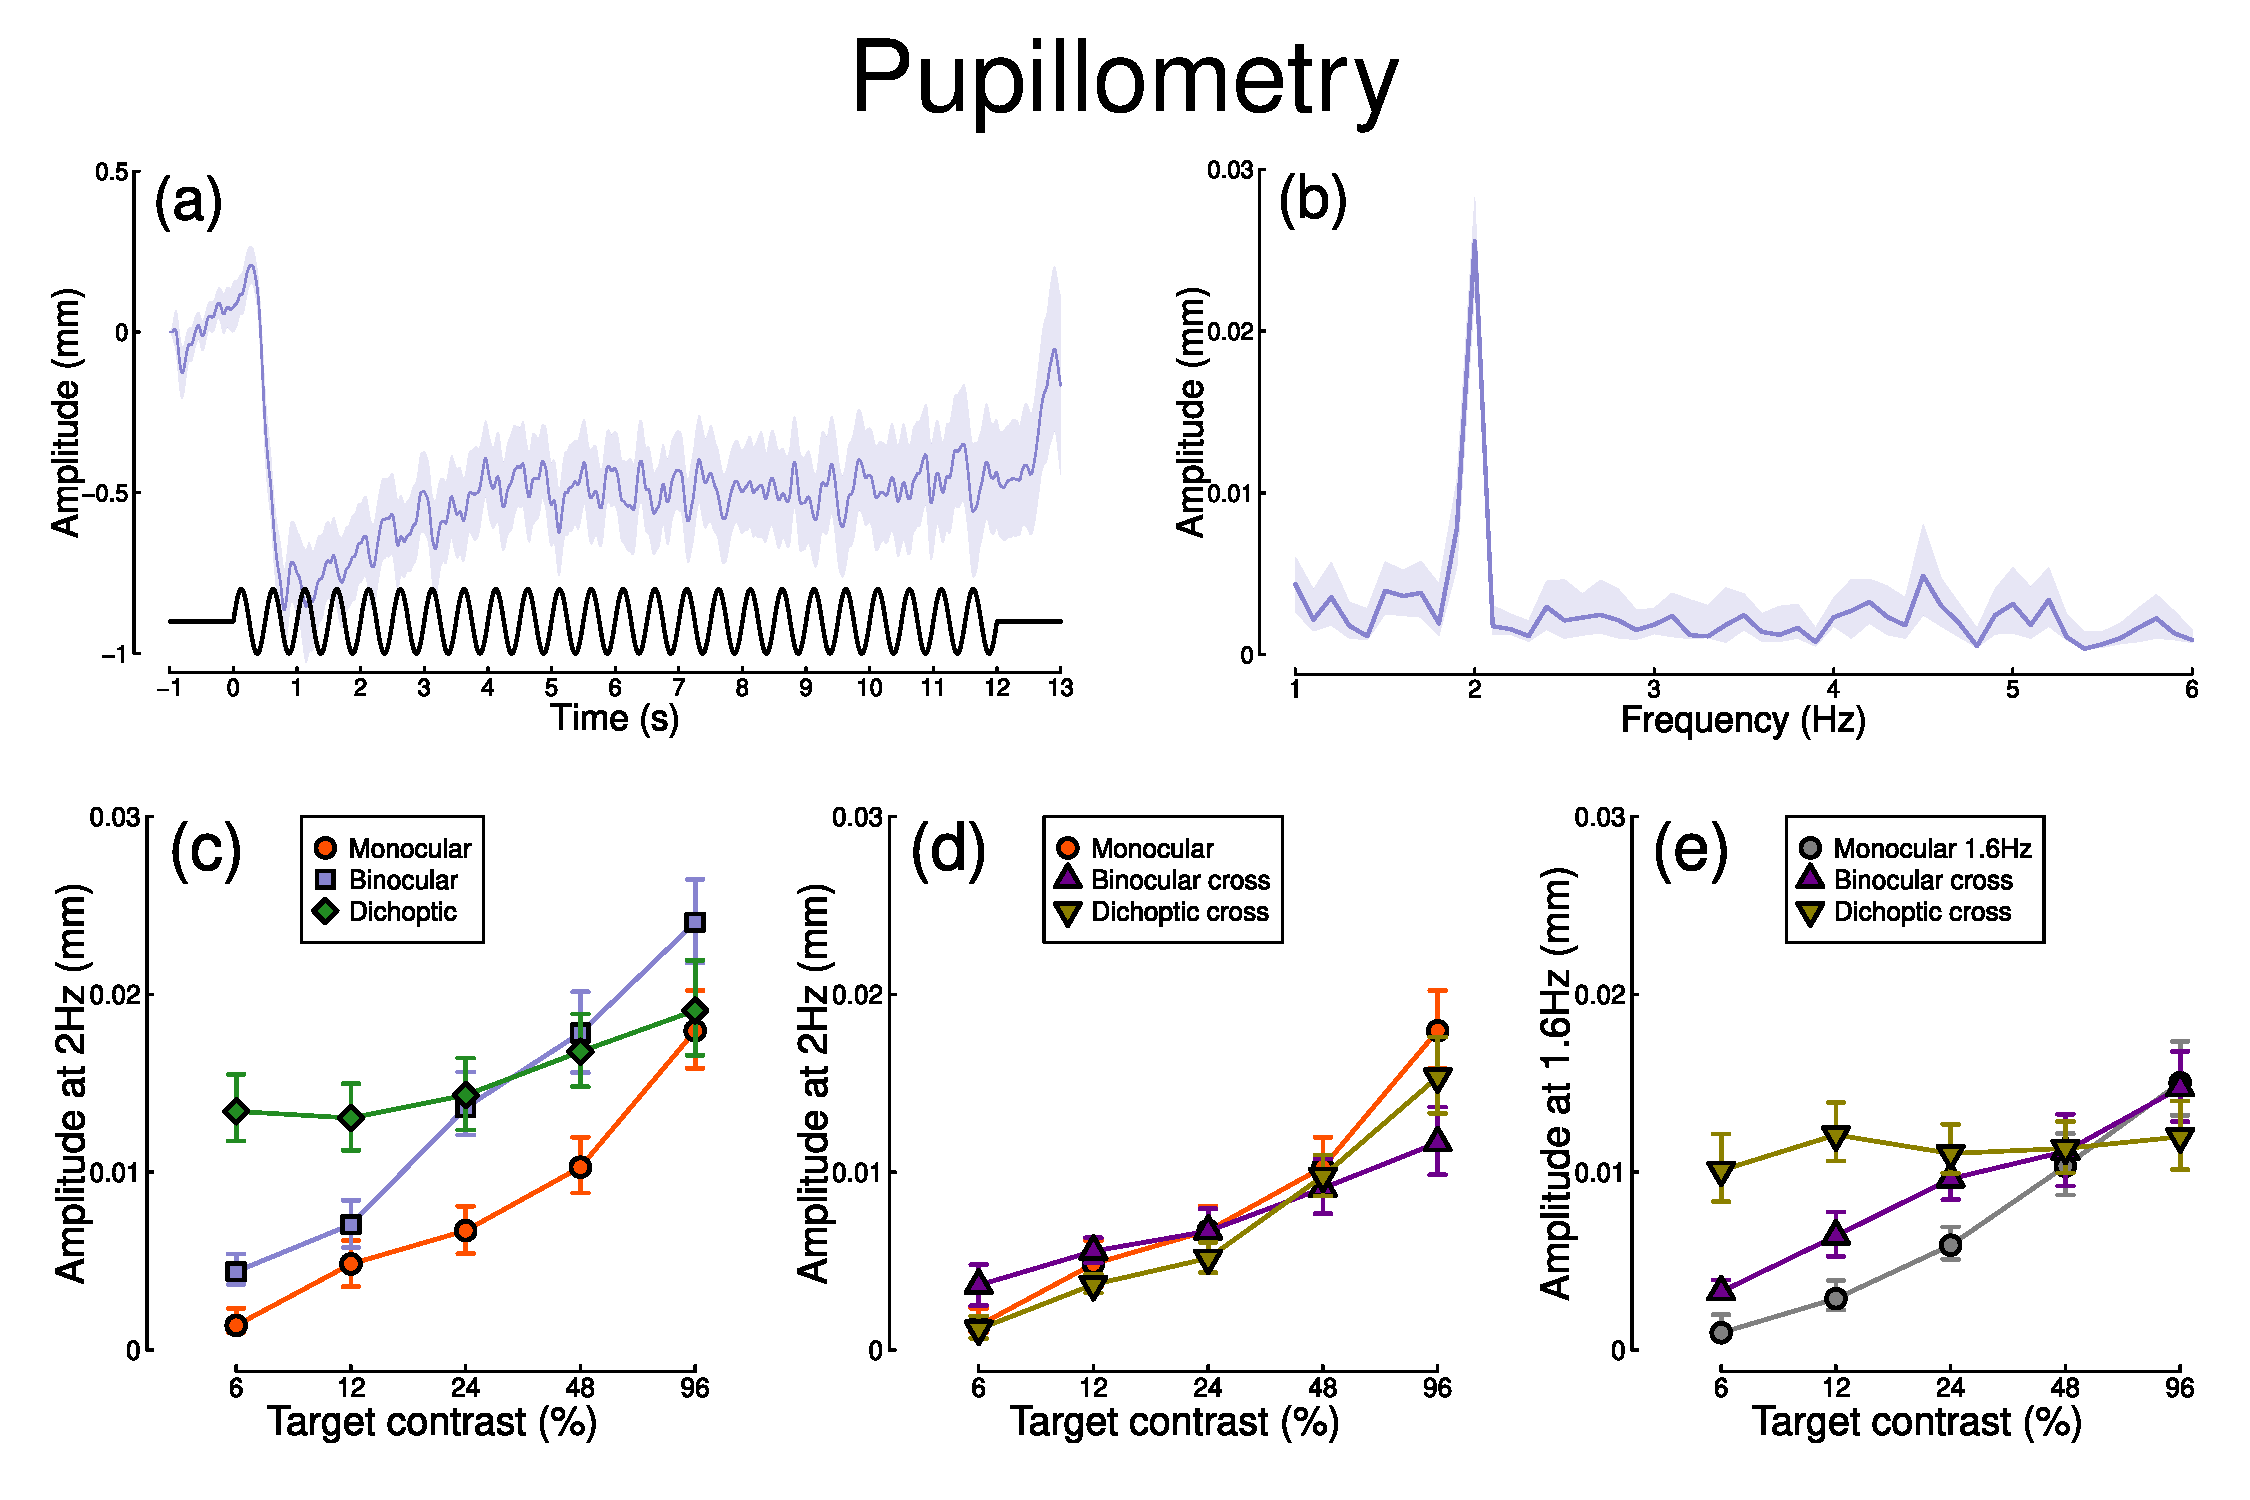
\includegraphics{local/Figures/pupildata} 

}

\caption{Summary of pupillometry results for N=30 participants. Panel (a) shows a group average waveform for binocular presentation (low pass filtered at 5Hz), with the driving signal plotted at the foot. Panel (b) shows the average Fourier spectrum. Panels (c,d) show contrast response functions at 2Hz for different conditions. Panel (e) shows contrast response functions at 1.6Hz for three conditions. Shaded regions and error bars indicate bootstrapped standard errors.}\label{fig:pupildata}
\end{figure}

\begin{figure}

{\centering 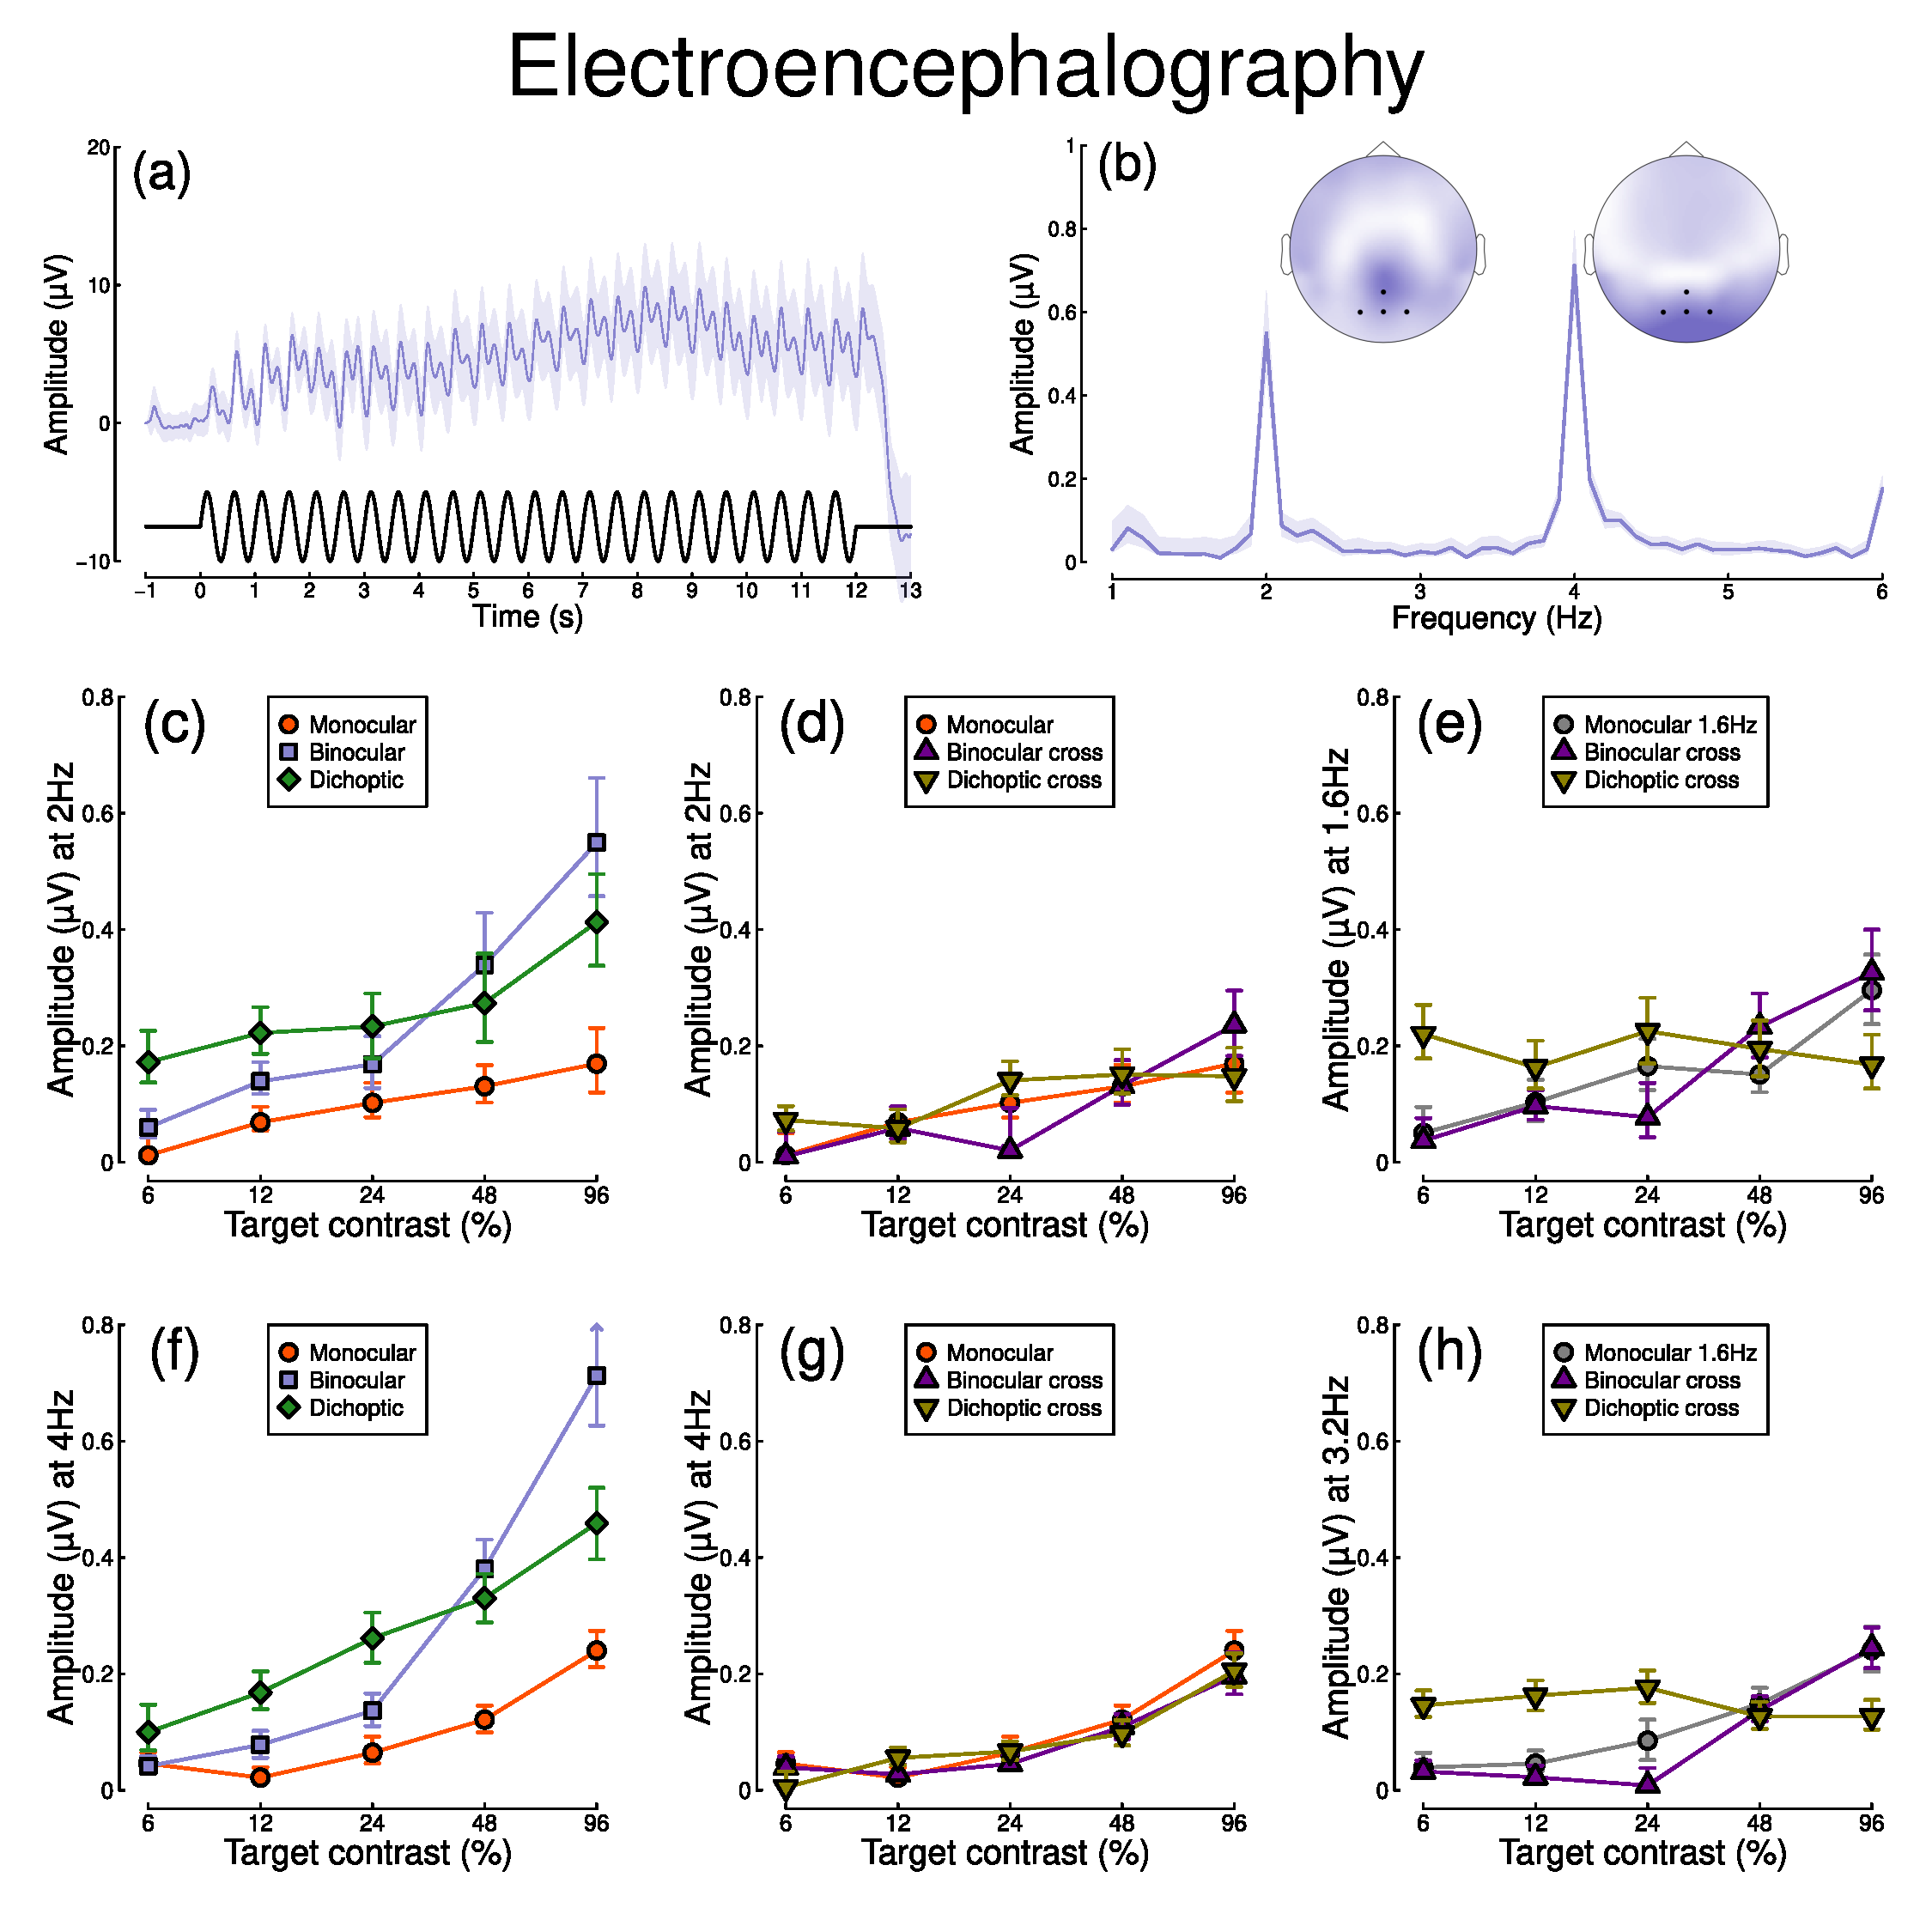
\includegraphics{local/Figures/EEGdata} 

}

\caption{Summary of EEG results for N=30 participants. Panel (a) shows a group average waveform for binocular presentation (low pass filtered at 5Hz), with the driving signal plotted at the foot. Panel (b) shows the average Fourier spectrum, and inset scalp distributions. Black dots on the scalp plots indicate electrodes Oz, POz, O1 and O2. Panels (c,d) show contrast response functions at 2Hz for different conditions. Panel (e) shows contrast response functions at 1.6Hz for three conditions. Panels (f-h) are in the same format but for the second harmonic responses. Shaded regions and error bars indicate bootstrapped standard errors.}\label{fig:EEGdata}
\end{figure}

\hypertarget{experiment-2}{%
\subsection{Experiment 2}\label{experiment-2}}

\begin{figure}

{\centering 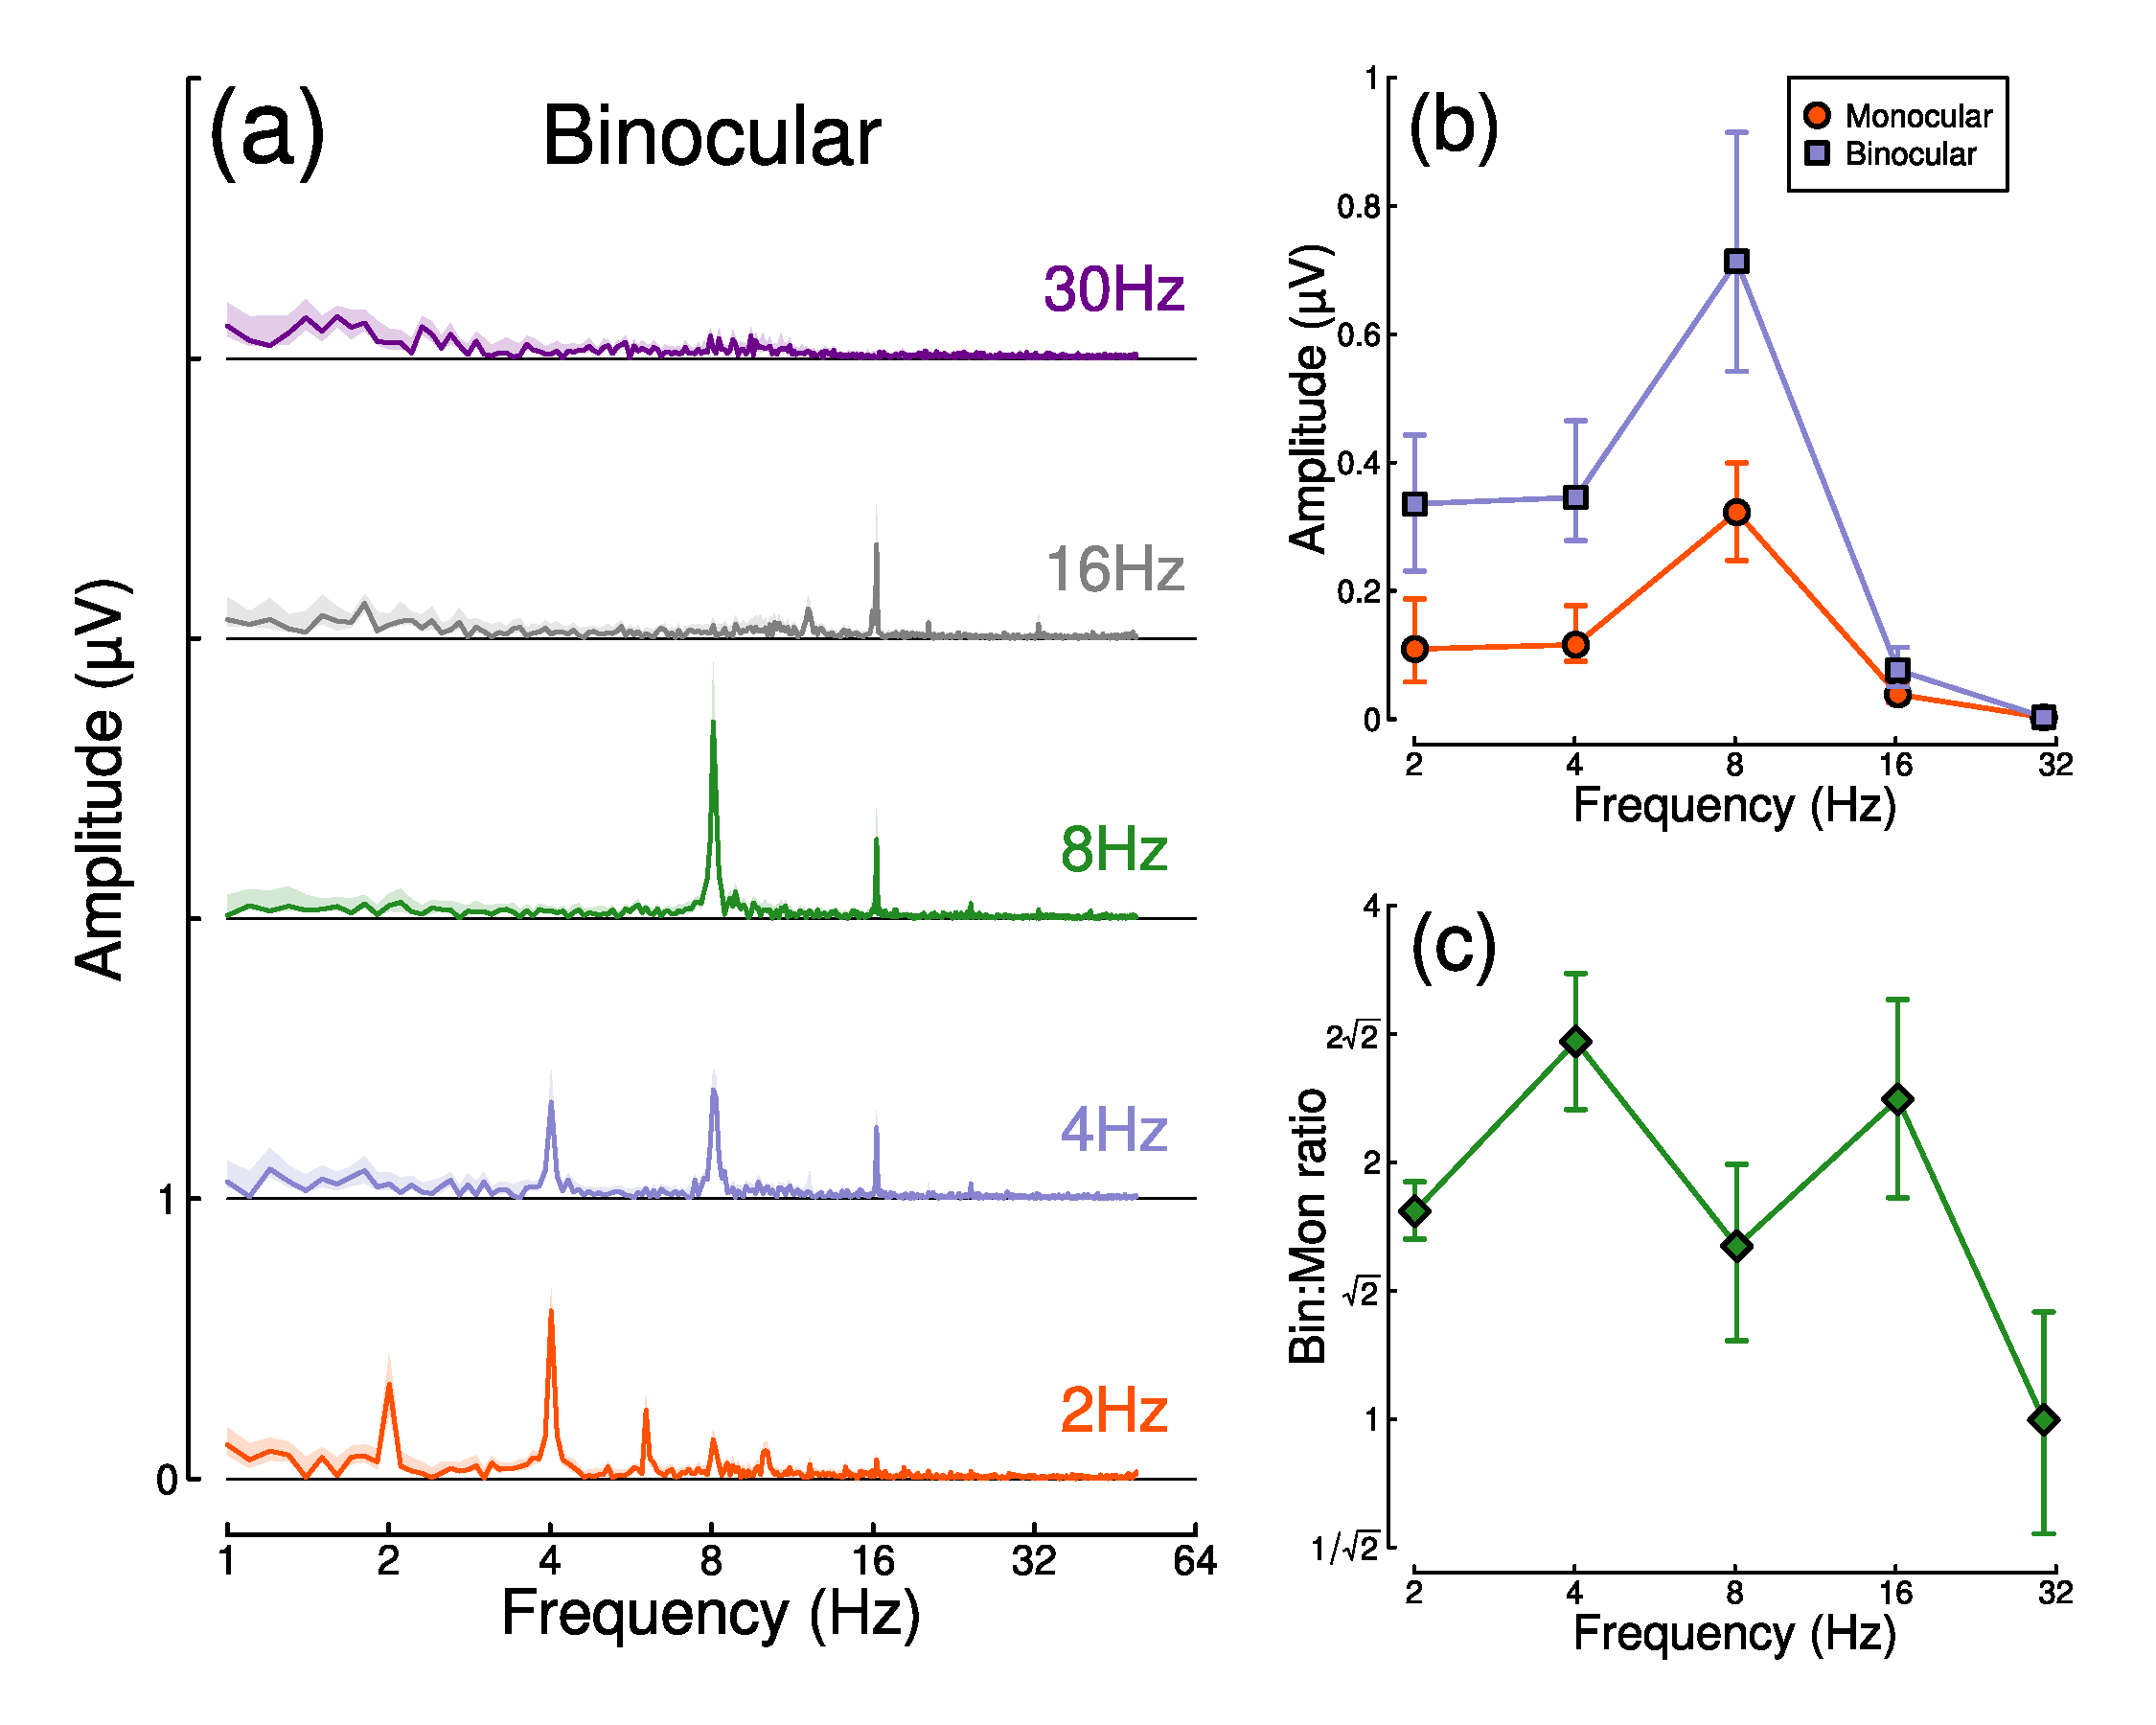
\includegraphics{local/Figures/TFdata} 

}

\caption{Binocular facilitation at different temporal frequencies. Panel (a) shows Fourier spectra for responses to binocular flicker at 5 different frequencies (offset vertically for clarity). Panel (b) shows the response at each stimulation frequency for monocular (red) and binocular (blue) presentation. Panel (c) shows the ratio of binocular to monocular responses. Error bars and shaded regions indicate bootstrapped standard errors.}\label{fig:TFdata}
\end{figure}

\hypertarget{experiment-3}{%
\subsection{Experiment 3}\label{experiment-3}}

\begin{figure}

{\centering 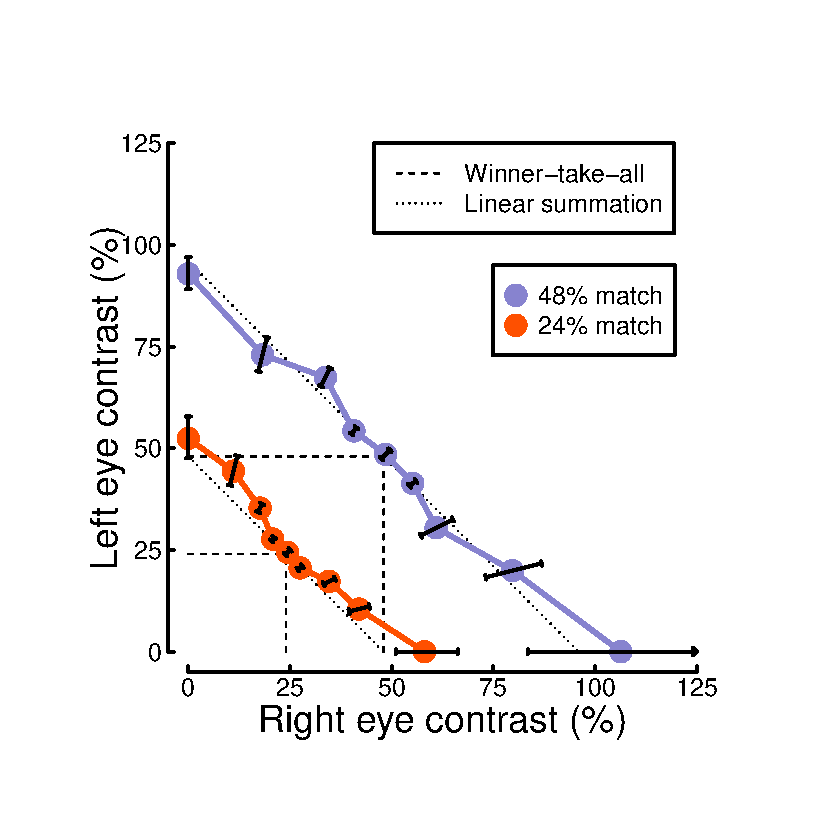
\includegraphics{local/Figures/matchingdata} 

}

\caption{Contrast matching functions. Dotted and dashed lines are predictions of canonical summation models with a linear exponent (dotted) or an infinite exponent (dashed). Error bars indicate the standard error across participants (N=10), and are constrained along radial lines converging at the origin.}\label{fig:matchingdata}
\end{figure}

\hypertarget{computational-modelling}{%
\subsection{Computational modelling}\label{computational-modelling}}

\begin{figure}

{\centering 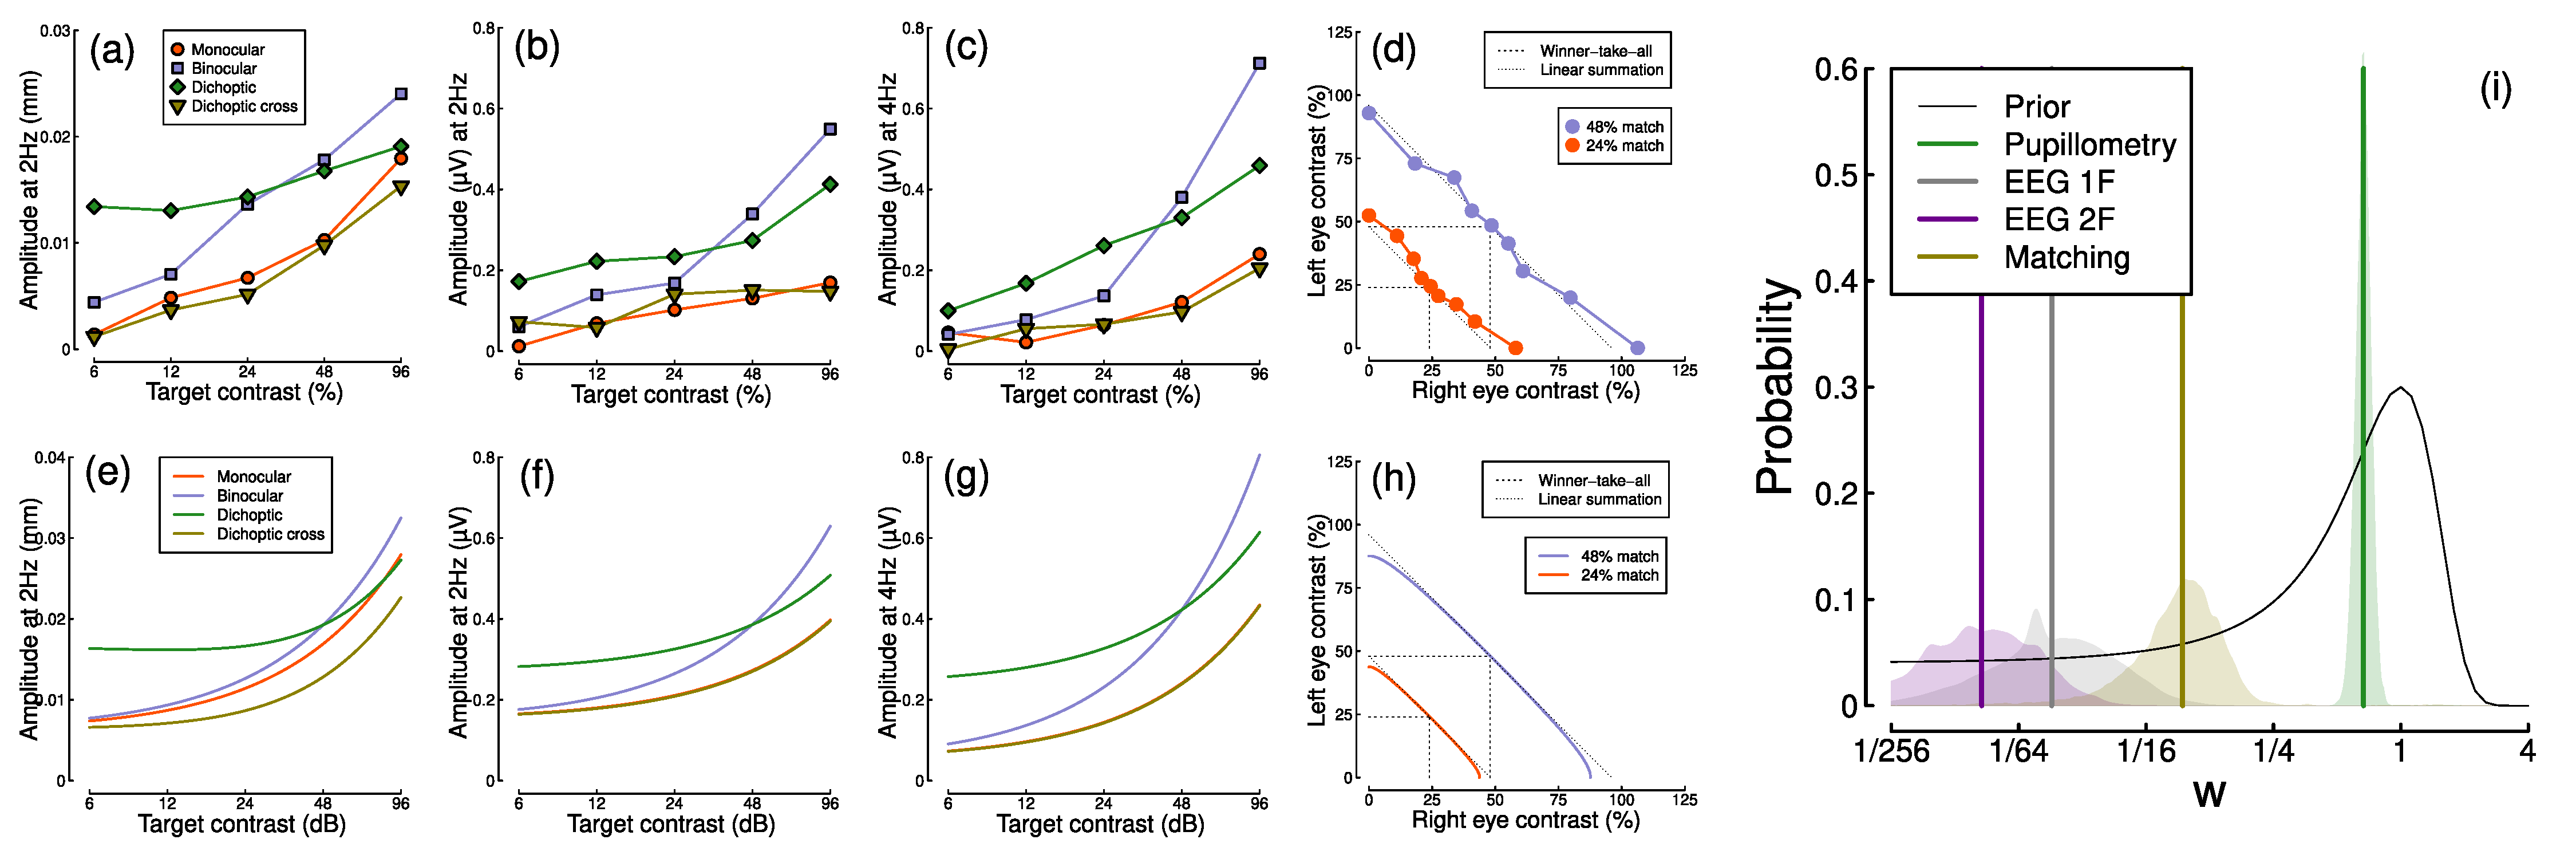
\includegraphics{local/Figures/modelfigure} 

}

\caption{Summary of computational modelling. Panels (a-d) show model behaviour for our four main data set, pupillometry (a), first harmonic EEG responses (b), second harmonic EEG responses (c) and contrast matching (d). Panel (e) shows the posterior probability distributions of the interocular suppression parameter for each of the four model fits. The pupillometry distribution (green) is centred about a substantially higher suppressive weight than for the other data types (note the logarithmic x-axis). The black curve shows the (scaled) prior distribution for the weight parameter.}\label{fig:modelfigure}
\end{figure}

\begin{table}

\caption{\label{tab:paramtable}Summary of median parameter values.}
\centering
\begin{tabular}[t]{l|c|c|c|c}
\hline
Data set & Z & k & w & Rmax\\
\hline
Pupillometry & 2.73 & 0.01 & 0.60 & 0.00022\\
\hline
EEG 1F & 2.09 & 0.15 & 0.02 & 0.00336\\
\hline
EEG 2F & 3.39 & 0.07 & 0.02 & 0.00312\\
\hline
Matching & 0.22 & 5.06 & 0.09 & -\\
\hline
\end{tabular}
\end{table}

\hypertarget{discussion}{%
\section{Discussion}\label{discussion}}

\hypertarget{references}{%
\section*{References}\label{references}}
\addcontentsline{toc}{section}{References}

\hypertarget{refs}{}
\begin{CSLReferences}{1}{0}
\leavevmode\vadjust pre{\hypertarget{ref-Baker2021}{}}%
Baker DH. 2021. Statistical analysis of periodic data in neuroscience. \emph{Neurons, Behavior, Data analysis, and Theory} \textbf{5}. doi:\href{https://doi.org/10.51628/001c.27680}{10.51628/001c.27680}

\end{CSLReferences}

\end{document}
